\documentclass[12pt,a4paper]{scrreprt}

%\usepackage{fontspec}
\usepackage{geometry}
\usepackage{mathtools}
\usepackage[english]{babel}
\usepackage{longtable,booktabs}
\usepackage{grffile}
\usepackage{graphicx}
\usepackage{titlesec}
\usepackage{capt-of}
\usepackage{newtxtext,newtxmath}

%\setlength{\leftskip}{25pt}
% Make links footnotes instead of hotlinks
%\renewcommand{\href}[2]{#2\footnote{\url{#1}}}

% No paragraph indentation
% and set space between paragraphs
\setlength{\parindent}{0pt}
\setlength{\parskip}{0.5em plus 1pt minus 1pt}
\setlength{\emergencystretch}{3em} % Prevent overfull lines
% Chapter: 0, section: 1, subsection: 2 etc
\setcounter{secnumdepth}{2}
\setcounter{tocdepth}{2}

\begin{document}
\pagenumbering{roman}
\begin{titlepage}
  \begin{center}

    
\includegraphics[width=40mm]{tu}\par\vspace{0.8cm}
    \textsc{\LARGE Tribhuwan University}\\[1cm]
    \textsc{\bfseries INSTITUTE OF ENGINEERING}\\
    \textsc{\bfseries PULCHOWK CAMPUS}\\
    \textsc{Pulchowk, Lalitpur}\\
    \vspace{0.8cm}

    \textsc{\Large A Case Study}\\[0.5cm]
    \textsc{On}\\
    {\huge \bfseries Paila Technology\\[0.4cm]}

    \vfill
    {\Large \bfseries Submitted By:\\}
    \noindent\makebox[\textwidth]{%
      \begin{tabular}{lr}%
        Aashutosh Poudel & \texttt{072BCT502}\\
        Dinesh Bhattarai & \texttt{072BCT512}\\
        Krishna Upadhyay & \texttt{072BCT517}\\
        Rupesh Shrestha  & \texttt{072BCT530}\\
        Simon Dahal  & \texttt{072BCT538}\\
        Yogesh Rai  & \texttt{072BCT548}\\
    \end{tabular}}\\[1cm]

    {\Large \bfseries Submitted To:\\}
    \textsc{Department of Mechanical Engineering} \\
    \textsc{Lalitpur, Nepal}
    \\[1cm]

    \vfill

    {\large \today}

  \end{center}
\end{titlepage}

\chapter*{Acknowledgements}
\thispagestyle{empty}
We would like to express our deepest gratitude to Prof. Shyam Krishna Joshi, honorable Professor for Organization and Management course, for his invaluable assistance, proper guidance and immense support to make us understand the core concept of Organization and Management and also encouraging us to do this case study on field.

Furthermore, we would also like to express our gratitude to Paaila Technology for not only allowing us to perform the study but also for helping us in all manners possible. Specifically, we would like to thank Mr. Wasim Akram Khan, Co-founder and Software Engineer and Mr. Dip Kamal Bhusal, CCO and Co-founder at Paaila Technology for dedicating their invaluable time and efforts towards this study and assisting us in the endeavor. Lastly, we would like to thank all our seniors, friends and family members for their support and suggestions.

- Team Members

\clearpage
\tableofcontents
\listoffigures
\listoftables
\clearpage
\pagenumbering{arabic}

\chapter{Introduction}
"Paila Technology", first of its kind in Nepali market, is a robotics and AI startup established on December 12, 2016 by Bijay Raut along with five other engineering graduates from IOE, Pulchowk Campus. The company started with a core team of seven members and the team has grown ever since. The company aims to produce world class robotics and industrial automation products that are suitable for businesses.
The company started with Automatic Dhara, automation for homes and have now transitioned into robotics by presenting their flagship project Pari, a robot for Nepal SBI Digital InTouch branch at Durbar Marg. Pari is a product that created a new market segment of robotics in Nepali market.

Paila is an entrepreneurial venture started with the prime motive to meet the demands of the market by developing a viable business model around some innovative products, services processes and platforms integrated with Artificial Intelligence and Robotics. The business model was a huge success in context of Nepal and the customerbase of the company is on rise. In a short span of time, the company has delivered products and services to some of the biggest names in the country including SBI Nepal Limited, nLocate, Gyani Traders and more to count.

\section{Vision}
The primary vision of "Paaila" can be considered as production of human friendly robots and to aid in the technological development of the country by embracing AI in different fields. It wants to aid other companies in integrating AI in their products as well to make AI and robotics available to everyone.

\section{Objectives}
The major objectives set by the company are:
\begin{enumerate}
  \item Be the best workplace for robotics and AI
  \item Be the best option for businesses seeking robotics Services
  \item Help Nepali companies integrate AI into their products and services.
\end{enumerate}

\chapter{Products and Services}

\section{Artificial Intelligence}
  Paaila Technology has invested a lot in robotics as a result it has to invest in AI too. 
  It has been working on various Artificial Intelligence and Machine Learning projects. Some of them
  are described below.

  \subsection{Recommendation System}
  Online ecommerce sites get benefitted when they can predict what users want and show them directly among their vast
  supply of products. Recommendation systems provide this capability to them. Paila has been aiding businesses grow using this technology.

  \subsection{Nepali Speech Recognition}
  This service is Speech to Text service that can transcribe audio. It can generate caption for videos
  or audio which can be further processed using Natural Language Processsing. This tool specifically deals with
  Nepali language.
  
  \subsection{Nepali Text To Speech}
  Although Text To Speech has matured, it is not on par with human voice. Moreover, the landscape is uneven accross different languages.
  This service tries to bridge the gap and make Nepali language a first class citizen in the field. The tool is found to be accessible to 
  hearing impaired audience. It has been demonstrated to turn text books to audio books in low cost and reliable manner.
  
  \subsection{Query Answering System}
  This service provides intelligent question answering helping people find correct answer easily and fast.
  It has been helping in intelligent communication with customers to businesses. It can answer all the queries while maintaining a record of the nature
  of conversation, topic and other information so that future decisions can be taken
  based on it to improve business performances. 


\section{Variable Frequency Drive}
\begin{enumerate}
  \item Introduction \\
    A Variable Frequency Drive (VFD) is a type of motor controller that drives an electric motor by varying the frequency and voltage supplied to the electric motor. Other names for a VFD are variable speed drive, adjustable speed drive, adjustable frequency drive, AC drive, and inverter. As the application's motor speed requirement change, the VFD can simply turn up or down the motor speed to meet the speed requirement.

  \item Working\\
    The first stage of a Variable Frequency AC Drive, or VFD, is the Converter. The converter is a comprised of six diodes, which are similar to check values used in plumbing systems. They allow current to flow in only one direction; the direction shown by the arrow in the diode symbol. For example, whenever A-phase voltage (voltage is similar to pressure in plumbing systems) is more positive than B or C phase voltages, then that diode will open and allow current to flow. When B-phase becomes more positive than A-phase, then the B-phase diode will open and the A-phase diode will close. The same is true for the 3 diodes on the negative side of the bus. Thus, we get six current "pulses" as each diode opens and closes. This is called a "six-pulse VFD", which is the standard configuration for current Variable Frequency Drives.

    \begin{center}
        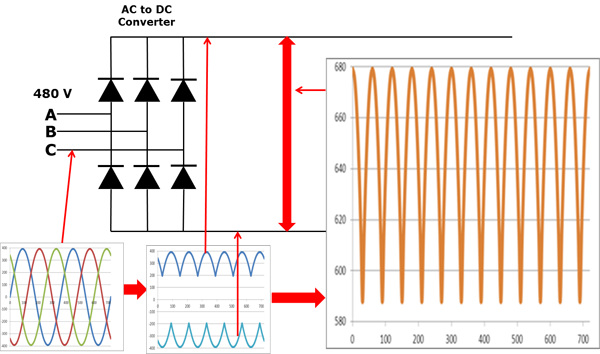
\includegraphics{vfd1}
        \captionof{figure}{Converter in a VFD}
    \end{center}

    If the drive is operating on a 480V power system, then the 480V rating is "rms" or root-mean-squared. The peaks on a 480V system are 679V. The VFD dc bus has a dc voltage along with an AC ripple. The voltage runs between approximately 580V and 680V.

    \begin{center}
        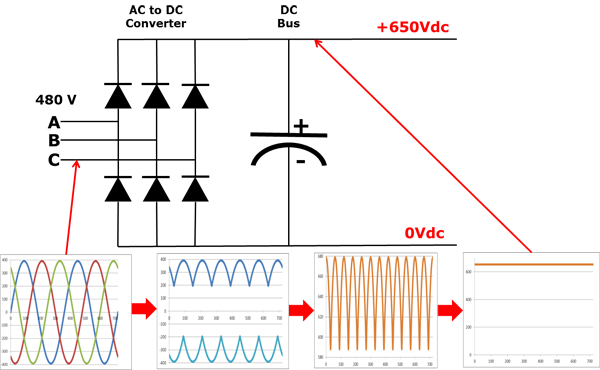
\includegraphics{vfd2}
        \captionof{figure}{Converter with DC Bus in a VFD}
    \end{center}

    A capcitor is added to get rid of the AC ripple on the DC bus. A  capacitor operates in a similar fashion to a reservoir or accumulator in a plumbing system. This capacitor absorbs the ac ripple and delivers a smooth dc voltage. The AC ripple on the DC bus is typically less than 3 Volts. Thus, the voltage on the DC bus becomes "approximately" 650VDC. The actual voltage will depend on the voltage level of the AC line feeding the drive, the level of voltage unbalance on the power system, the motor load, the impedance of the power system, and any reactors or harmonic filters on the drive. \\

    The diode bridge converter that converts AC-to-DC, is sometimes just referred to as a converter. The converter that converts the dc back to ac is also a converter, but to distinguish it from the diode converter, it is usually referred to as an "inverter". It is common in the industry to refer to any DC-to-AC converter as an inverter.

    \begin{center}
        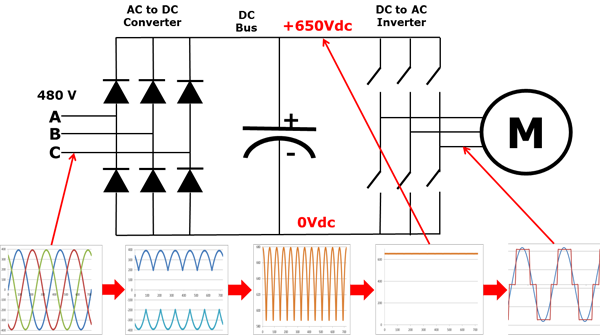
\includegraphics{vfd3}
        \captionof{figure}{Converter, DC Bus, and inverter in a VFD}
    \end{center}

    When one of the top switches in the inverter is closed, that phase of the motor is connected to the positive dc bus and the voltage on that phase becomes positive. When one of the bottom switches in the converter is closed, that phase is connected to the negative dc bus and becomes negative. Thus, any phase on the motor can be made positive or negative at will and can thus generate any frequency. Also, any phase can be made positive, negative, or zero.

    \begin{center}
      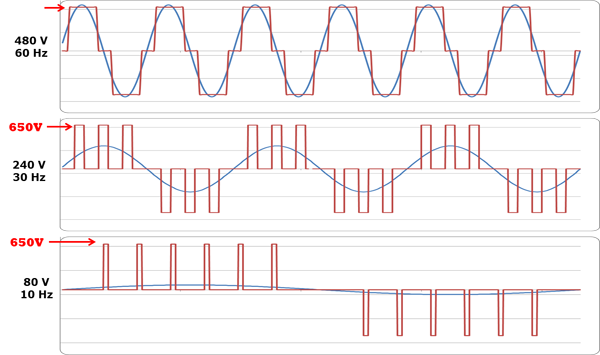
\includegraphics{vfd4}
      \captionof{figure}{Output response of a VFD}
    \end{center}

    The output from the VFD is of "rectangular" wave form. VFD's do not produce a sinusoidal output. This rectangular waveform would not be a good choice for a general purpose distribution system, but is perfectly adequate for a motor.

  \item Benefits
    \begin{itemize}
      \item Electric motor systems are responsible for more than 65\% of the power consumption in industry. Optimizing motor control systems using VFDs can reduce energy consumption and energy costs.
      \item Using VFDs, equipments can be operated at optimimum and efficient speeds, thereby extending the equipment life and reducing maintenance costs.
    \end{itemize}

  \item VFDs by Paila Technology
    \begin{itemize}
      \item Current Market in Nepal
        \begin{itemize}
          \item VFDs for \textit{Allo} thread producing machine
          \item VFDs for changing speed of DC motors in tempos
          \item VFDs for automatic brick producing machines
        \end{itemize}

      \item Features
        \begin{itemize}
          \item Customizable for different applications
          \item Production against possible drive failures
          \item Quality support and maintenance
          \item Compatible with single phase supply
          \item Made for Nepali Industries
        \end{itemize}

      \item Technical Specification
        \begin{center}
          \begin{tabular}{|l|l|}
            \hline
            Parameters & Values \\
            \hline
            Input Voltage & 380 to 480V 3ph or 230V single phase \\
            Input Frequency & 50Hz or 60Hz \\
            Output Voltage & 0 to rated line voltage \\
            Output Frequency & 0.5Hz to 200Hz \\
            Switching Frequency & 3kHz to 12kHz \\
            Rated Power & 0.5HP to 15 HP \\
            Control Method & Linear V/f \\
            Display & 7-segment or Alphanumeric LCD \\
            Digital Inputs & 5V DC optically isolated \\
            Analog Inputs & 0 to 5V \\
            \hline
          \end{tabular}
        \end{center}
    \end{itemize}
    Resources: https://www.vfds.com/blog/what-is-a-vfd
\end{enumerate}
\chapter{Organization Structure}

An organizational structure is a system that outlines how certain activities are directed in order to achieve the goals of an organization. These activities can include rules, roles and responsibilities. The organizational structure also determines how information flows from level to level within the company. For example, in a centralized structure, decisions flow from the top down, while in a decentralized structure, the decisions are made at various levels. \\

Organizational structure defines a specific hierarchy within an organization, and businesses of all shapes and sizes use it heavily. A successful organizational structure defines each employee's job and how it fits within the overall system. This structuring provides a company with a visual representation of how it is shaped and how it can best move forward in achieving its goals. \\

At its highest level, an organizational structure is either centralized or decentralized. Traditionally, organizations have been structured with centralized leadership and a defined chain of command. The military, for example, is an organization famous for its highly centralized structure, with a long and specific hierarchy of superiors and subordinates. However, there has been a rise in decentralized organizations, as is the case with many technology startups. This allows the companies to remain fast, agile and adaptable, with almost every employee receiving a high level of personal agency. \\

Paaila Technology is a fast paced company with core focus on AI, robotics, and industrial automation. In a short span of time, it has delivered products and services to some of the biggest brands in the country – SBI Nepal Limited, nLocate, Gyani Traders and many more. Paaila's popular flagship product 'Pari', a humanoid robot was deployed in providing customer service at SBI Bank in 2017. At its early stage, Paaila has captured the imagination of local Nepali market and acquired notable media attention by providing customer service through a humanoid robot. \\

\begin{center}
    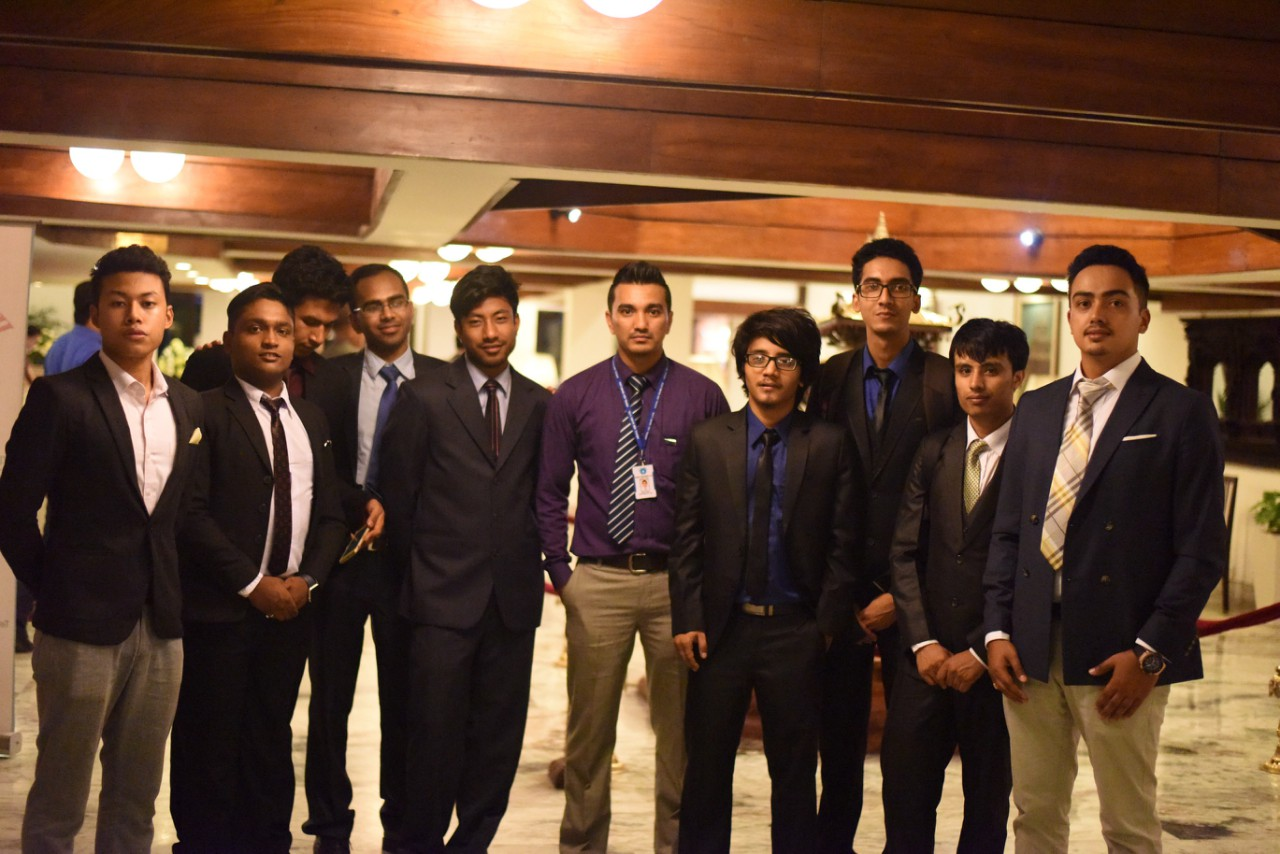
\includegraphics[scale=0.45]{paila-group}
    \captionof{figure}{The founding members of Paila Technology src:startupsnepal.com}
\end{center}

Being an entrepreneurial venture started with a newly emerged concept in the marketplace, the prime motive of the advent of Paaila was to meet the demands and needs of the market by developing innovative products, services, processes and platforms relating to Artificial Intelligence and Robotics in context of Nepal. Being a startup, the company was initially formed with a small team of 7 members with a common interest. The company has a team of co-founders to secure key-skills, financial
resources, and other elements to conduct research on the target market while there are technical experts from different fields of engineering working together to think and develop the new ideas and innovative product concepts. In addition, the company consists of a management team which is responsible for major decisions on company’s plans, organization, staffing, coordination and control. \\

\begin{enumerate}
    \item \textbf{Management Model} \\
    A hybrid model of management comprising of a mixture of two management models, hierarchical and team efforts management model is followed. The overall structure can be taken as a hierarchy with Chairperson on the top, followed by the Chief Executive Officer(CEO), co-founders, other chief officers, engineers and finally the interns, staffs and other contract-based workers. But, to ensure better execution of projects, the organization follows a team efforts management model where the organization comprises of different teams based on the tasks. Individual groups give their best to the projects, while the head monitors the performance of all groups.

    \begin{center}
        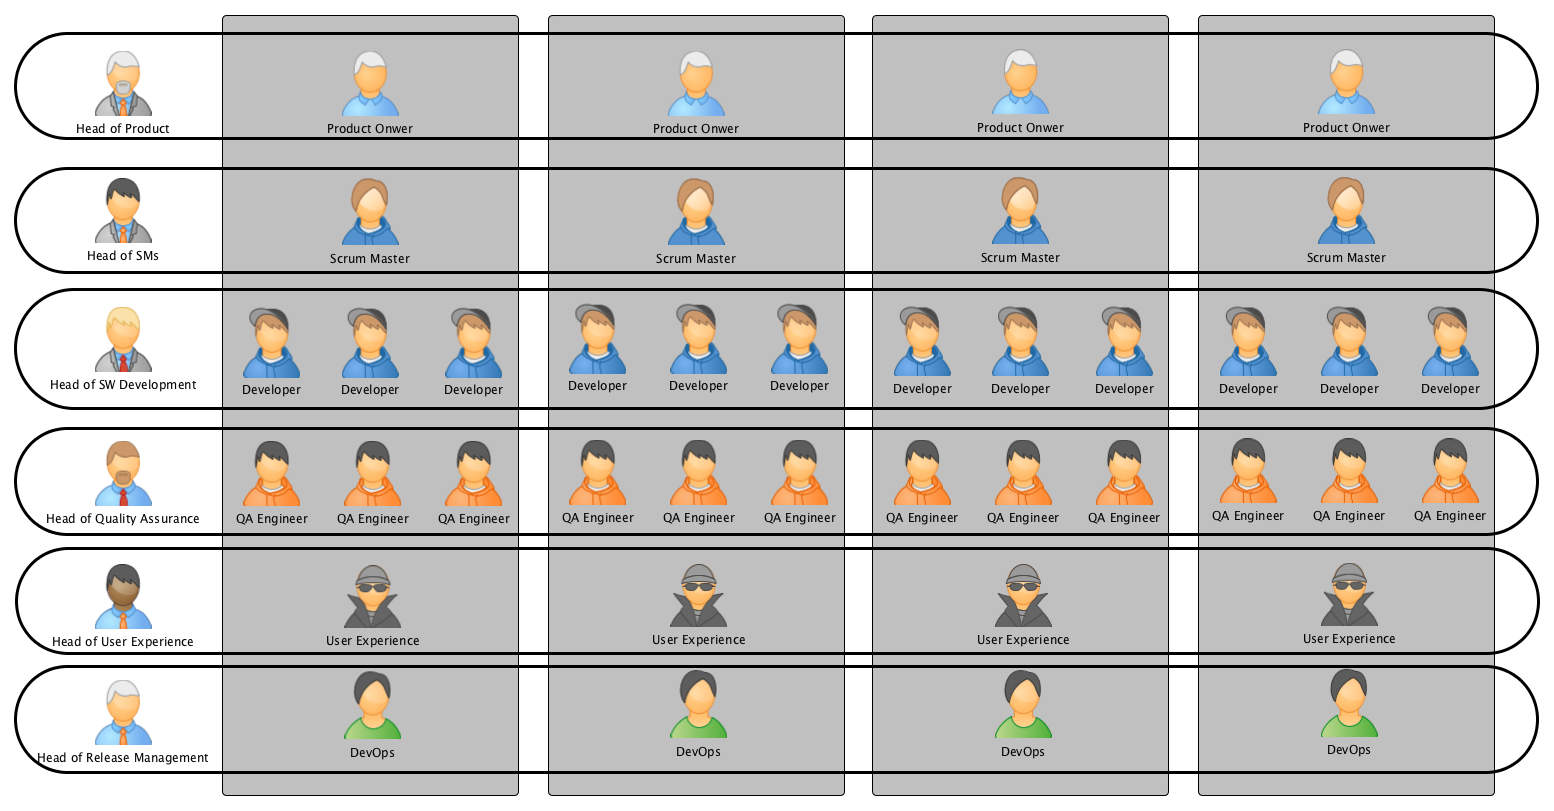
\includegraphics[scale=0.28]{team-based-MM}
        \captionof{figure}{Team based Management Model}
    \end{center}

    \item \textbf{Line Organization} \\
    According to this type of organization, the authority flows from top to bottom in a concern. The line of command is carried out from top to bottom. This is the reason for calling this organization as scalar organization which means scalar chain of command is a part and parcel of this type of administrative organization. In this type of organization, the line of command flows on an even basis without any gaps in communication and co-ordination taking place. \\
    This form of organization promotes greater decision making as every organization units is directly involved in the day-to-day business activities of the company. There is direct vertical links between the different level or layer of the company. Although the top-level management team is responsible for giving the major verdicts on company’s next steps, the chief officers in advisory of sales and marketing officer and operations manager as well as the members of the engineering team who have better knowledge and expertise regarding technical aspects too are free to express their views and advice to the top managerial level. The Line Organizational structure simplify and clarify authority, responsibility and accountability relationship among the different layers in the organization. It promotes fast decision making.

    \begin{center}
        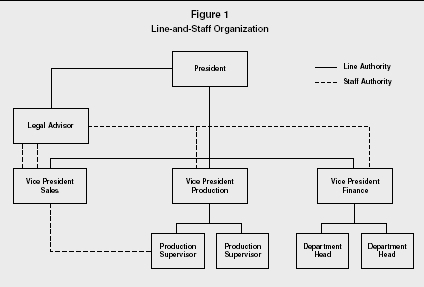
\includegraphics{line-org.jpg}
        \captionof{figure}{Line Organization}
    \end{center}

    \item \textbf{Current Structure} \\
    The organization consists of the Chairman Mr. Binay Raut as the Head of the Organization and a Chief Executive Officer. Under the CEO, the company has a team of 6 co-founders along with 1 extra stakeholder making it partnership organization of 7 investors. The major decisions are made by the management meeting. The decision to purchase a highly costly product includes the involvement of CEO and the 7 stakeholders. Other decisions on project plan, budget plans for project, project deadlines, progress of projects are all done on the basis of conclusions derived from the meetings held compulsorily on a weekly basis on the presence of the co-founders' team, chief officers team, sales officer, operations manager and all the engineers of different engineering teams.

    The decisions of purchase and procurement like hardware purchases, purchases of sensors, microcontrollers, etc. are made depending on their level of expense. For minor purchases, the development teams keep track of expenditures and finally present the bills of their entire expense at the next meeting while in case of major purchase, decisions are made by the stakeholders and the management on whether or not to buy the product and at the reasonable price. The entire team is responsible for public relations management as any one of the members of the company who may be best suitable is sent for the communication with external agents based on the nature of the agent, task to be done and the required expertise. The member then mandatorily updates the entire team about all the highlights of his meet with the agent and provides the contact information via a group chat in a messaging platform called \textit{Slack} so that the follow up of the task can later be possible by any of the team members. All of the information on the projects plans, project documentations, progress reports, etc. are shared to all of the members involved in a particular project via Google Drive while weekly deadlines and milestones to be completed are discussed on \textit{Slack}.

    \item \textbf{Block Diagram} \\
    \begin{center}
        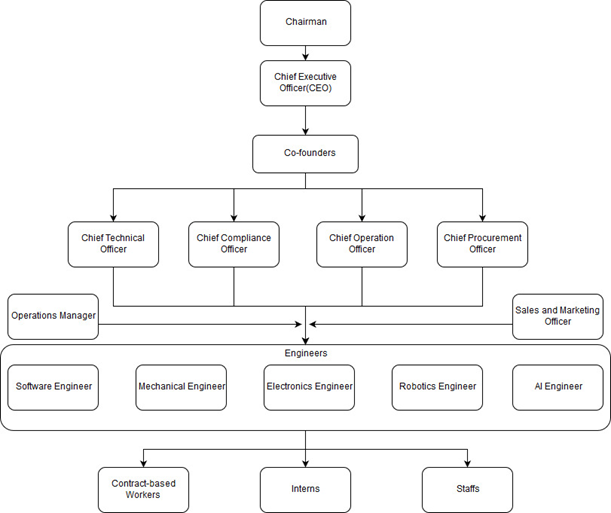
\includegraphics[scale=0.7]{block-diagram.png}
        \captionof{figure}{Organization Hierarchy}
    \end{center}

    \item \textbf{Functional Structure} \\
    The overall structure of the organization can be categorized into four different levels. The levels although distinctly categorized may rather be taken as homologous in the sense that the top-level co-founders are also involved in the engineering team, the chief officers are also involved in the engineering team and so on. The four levels are as follows:

        \begin{enumerate}
            \item \textbf{Administrative level} \\
            The organization has a Chairperson and the Chief Executive Officer (CEO) at this level. They take major decisions of investments and public relations with other established companies like banks, telecommunications etc. They are responsible for the company's strategy and make the final call on resource allocations thereby guiding the organization to being more organized.

            \item \textbf{Management team} \\
            It consists of the 7 co-founders of the company who are designated with different posts such as the CTO, COO, CPO and CCO, the roles of each are described below:

            \begin{enumerate}
            \item \textbf{CTO (Chief Technical Officer)} is an executive position whose holder is focused on scientific and technical issues within an organization. Essentially, a CTO is responsible for the transformation of capital - be it monetary, intellectual, or political - into technology in furtherance of the company's objectives and decisions and maintenance of the project technology stack.

            \item \textbf{CCO (Chief Commercial Officer)} is also an executive-level role, with the holder being responsible for the commercial strategy and the development of an organization. It typically involves activities relating to marketing, sales, product development and customer service to drive business growth and market share.

            \item \textbf{COO (Chief Operations Officer)} is responsible for the daily operation of the company and routinely reports to the highest-ranking executive, i.e., the administration level. COO is also responsible for tackling with the obstacles and problems faced in the due course of project development such as resource and equipment unavailability as well as tracking each project's timeline and ensuring each deadline is met.

            \item \textbf{CPO (Chief Procurement Officer)} is an executive role focused on sourcing, procurement, and supply management for an enterprise.
            \end{enumerate}

            \item \textbf{Engineering team} \\
            The Engineering team includes a group of highly experienced and enthusiastic engineers from all fields of engineering like mechanical, computer, electronics, architecture and software all working together to create innovative ideas as products and services.

            \item \textbf{Staffs and Interns} \\
            The company has a few number of low level staffs with a few interns. The interns are rather treated as coworkers of the engineering team. Workers are rather hired on contract basis depending on the need of the project and type of expertise needed.


        \end{enumerate}

\end{enumerate}


\chapter{Personnel Management}
Paila Technology, which formally started on December 12, 2016, envisioned to produce world class robotics and industrial automation products that are suited for Nepali industries. Towards the end of 2014 when Binay Raut, the founding member and current CEO of Paila Technology, returned to Nepal after his MSc with a passion to innovate in the field of technology. Seven months later, he teamed with 5 engineering graduates of IOE, Pulchowk to start a commercial robotics company. Started with 7 core-team members, the company grown its size and reached a total of 25 employees including the Chairman, CEO, Co-founders, Stakeholders, Chief Technical Officer, Chief Procurement Officer, Chief Commercial Officer, Chief Operation Officer, engineers and interns.
\section{Recruitment, Selection and Training}
Similar to many other companies, the recruitment and selection process involve either an internship program or a training program that leads to full time employment at this organization or contract-based recruitment.
	\begin{itemize}
		\item \textbf{Intern:} Annually, about 3-4 months are allocated for internship for enthusiastic developers and students. It involves engineering students as well as computer science students or maybe even graduates looking for experience in professional work for their future. Currently, there are only a few number of interns working in the company to hone their skills in the field of AI, Robotics and NLP.
		\item \textbf{Full-time Employee:} According to the manpower planning and HR department, through the vacancy announcement, a full-fledged job is given to the applicant on the basis of their experience, caliber and achievement.
		\item \textbf{Contract-based Employee:} As per the needs of the organization, employees are hired on contract basis to carry out the projects. It is fully dependent on the needs of client, i.e. with the increasing demand from the clients, the number of employees getting involved in different projects in parallel increases. So, for the time being, the team expansion plans are totally relying on the need of the clients and market demands for the products of the company.
	\end{itemize}
	
The procedures involved in candidate selection are defined under following headings:
	\begin{itemize}
		\item \textbf{Call for Applicants:} Advertisements and vacancy announcements are circulated mostly through online media.
		\item \textbf{Application Collection:} The applications are received along with any supporting testimonials like a resume and other identification documents.
		\item \textbf{Resume Assessment:} The documents sent by the applicants along with CV are then analyzed by the senior engineers and project managers and the HR department to reduce the number of potential candidates for selection or screening candidates for the best fitting candidate.
		\item \textbf{Exam:} Based on the CV, the shortlisted candidates are supposed to appear for the written examination whereby computational and technical capabilities of the
candidates are tested.
		\item \textbf{Interview Process:} The ultimate part of the selection process involves multi-stage interviews. During an interview, HR Manager together with Senior Engineer assess
the technical skills along with the work ethics and attitude inherent in the candidate. Their dedication and efforts with teamwork is also evaluated thoroughly.
	\end{itemize}

In the starting phase of 3-4 months, the selected applicants will then have to go through
training sessions on respective fields so as to make them competent to work in real world.
\section{HR Divisions}
The comapny has following divisions or departments:
\subsection{Mechanical Division}
Mechanical and Electrical Engineers work under this division. They are responsible for disigning and building the robot body. The beautiful body of Pari is outcome of the efforts of these people.

\subsection{Embedded Division}
Electronics, AI and Robotics engineers work under this division to integrate hardware devices with software to create a piece of art.

\subsection{Language Processing}
Software engineers specialized in Natural Language Processing work under this division to create a human interface using speech and text, specializing in Nepali language. Due to large scarcity of datasets in the language, interns are mostly employed in web scraping.

\subsection{Operation Management}
Employees under this divsion oversee all other divisions to see if they are functioning properly. They work tirelessly to see if lack of lack of resource or manpower is hampering any deparment.

\section{Motivation}
\textit{Motivation is defined as the internal forces that impact the direction, intensity and persistence of a person’s voluntary choice of behavior.} The \textbf{direction} is indicative of the focus on the goals, the \textbf{intensity} of the bulk of effort allocated and \textbf{persistence} of the amount of time taken for the effort to be executed.

It is common that \textit{happy} and \textit{motivated} employees are confused with each other. These people may seem similar but there is fundamental difference between them. Happy people will keep the environment healthy and will always give a net profit but motivated ones, they are the ones with whom companies thrive. They are the ones who are productive, managed and invested. When enough of motivated employees are around, company starts to thrive and managers have easier time managing such people. 

Paila Technology seems to have attempted at its best level to motivate its employeees through its cool and amiable atmosphere. The company has got an edge advantage on employee motivation because AI is a relatively new field in Nepali markets and employess themselves are fascinated by the field. Moreover, the company has won three nationally recognized awards: \textbf{Best Startup Award}, \textbf{Most Innovative Product Award} and \textbf{Best Industry Award (Technology)} in a row and that's also in the first year of the company has created a great motivation for existing employees and newbies. Furthermore, Pari has gained enough popularity that all the people associated with it feel valuable themselves.

Financial aspect of the company also seems to be sound enough that the retention rate of the company is pretty good. Along with various means of recreation like planned excursions every six months give a releaf from hectic schedules and fill the mind with new zeal and enthusiasm to work more productively.
 
In a nutshell, the high popularity of the comapany in a short span and implementing cool gadgets in context of Nepal along with delivering quality product to businesses, employees do not only seem to be happy but also highly motivated.

\chapter{Finance Management}
\chapter{Software Engineering Methodology}

\chapter{Organizational Challenges}
\section{Lack of expertise and difficulty to retain them}
\section{Lack of raw materials}
\section{Insufficient training data-sets}

\chapter{Recommendation}
\section{Outsourcing}
\section{Extending HR base for better responsibility division}

\chapter{Conclusion}
\chapter*{References}
\bibliography{bibliography}
\end{document}
